\documentclass{article}
\usepackage{graphicx}
\begin{document}
	\section*{Notizen Datenbanken}
	\subsection*{15.04.2021}
	Einführung in die Veranstaltung. \\ \\
	ERM \\
	SQL \\
	Relationale Algebra \\
	Daten - Rohdaten, Messunggen, Fakten \\
	Informationen - gewonnene Erkenntnisse aus Rohdaten \\
	Daten - Informationen - Wissen \\
	DBMS - Datenbankmanagementsystem
	Anwendungen kommunizieren mit DBMS. \\
	Daten werden von DBMS verwaltet. \\
	Daten: strukturiert, semi-strukturiert, nicht strukturiert. \\
	Datenbanken speichert strukturierte Daten. \\
	Entscheidung:	Lokation - Größe - DBMS  \\
	Kommunikation nur mit DBMS nicht mit Datenbank direkt!!!!! \\
	Def. Kap 1 F 41 \\
	Datenbanken sind unabhängig vom Anwendungsprogramm. \\
	Funktionen: \\
	Große Datenmengen speichern. \\
	Forderungen: \\
	Effizienz  \\
	Data Warehouse Operational DB \\
	Relationale Datenbanken \\
	redundanzfreie Einmalspeicherung \\
	Jedes Tupel kommt nur einmal vor. \\
	Einfache Datentypen \\
	Objekt relationale Datenbanken \\
	OQL - Object Query Language \\
	XML DB \\
	XML Schema definiert Datenbank \\
	\subsection*{22.04.2021}
	Relationale Algebra \\
	Multimengentheorie \\
	Wiederholung Mengenoperationen \\
	Kartesisches Produkt \\
	Relationen \\
	Edgar F. Codd Urvater der relationalen Datenbanken. \\
	- ist Backslash \\
	Datenbanken lassen auf Union alle möglichen Ergebnisse zu \\
	Auch Duplikate \\
	Kopf: Attribut \\
	Rumpf: Tupel \\
	Innerhalb der n-Tupel ist die Reihenfolge nicht egal. \\
	Relationsschema \\
	Wenn Abweichung, angeben!! \\
	Domäne \\
	Studet(ID: Integer, name:String, Nachname:String) \\
	Einfache Datentypen \\
	Grad(Spaltenzahl), Kardinalität (Zeilenzahl) \\
	Mengenoperationen erfordern gleiche Attribute \\
	Es empfiehlt sich: gleiche Ordnung der Attribute \\
	Empfehlung Iwer: Reihenfolge der Attribute vor der Durchführung der Operation anpassen. \\
	Entfernungsoperatoren \\
	Projektion $\pi$ \\
	Enthält eine Teilmenge der Attribute von R \\
	(Verkleinern auf gewünschte Attribute) \\
	Sample: $\pi_{A1, A2, A3}(R)$
	Attribute klein schreiben \\
	Selektion: Auswahl mit Bedingung \\
	Bedingung muss ein boolescher Operator sein. \\
	\subsection*{29.04.2021}
	Multimengentheorie Duplikate sind erlaubt. \\
	Mengen \\
	Domänenschema einfach und vollständig \\
	$\sigma$ $\to$ verändert Kardinalität \\
	z.B. $\sigma_{b>1}$(R) \\
	$\delta$ entfernt alle Duplikate \\
	$\rho$ kann Relation oder die Attribute einer Relation umbenennen \\
	R(a,b,c) $\rho_{S_{c,d,a}}$(R) $\to$ S(c,d,a)
	S.a spricht Attribut a von S an. \\
	Erweiterte Projektion lässt auch Umbenennungen und Berechnungen zu \\
	Instanz einer Datenbank \\
	Operationenbaum \\
	expressiontree \\
	drafische Darstellung der auszuführenden Operationen auf eine Relation \\
	Tau ermöglicht Sortierung \\
	Sortierung lexikografisch aufsteigend. \\
	Tau enthält liste von Attributen nach denen Sortiert werden soll, erstes Sortierkriterium zuerst. \\
	Sortieren immer als letzte Operation. \\
	Kombinationsoperationen \\
	Unterschiedliche Daten verbinden mit Join \\
	Kreuzprodukt \\
	Alle Tupel werden mit allen anderen Tupel der anderen Relation verbunden \\
	Natural Join \\
	Attribute mit gleichem Namen werden verbunden \\
	Tupel werden Verbunden wenn bei gleichem Attribut gleicher wert enthalten. \\
	Nur Zusatzattribute werden übernommen. \\
	Bei mehreren gleichen Attributen müssen auch die Werte aller gleichen Attribute gleich sein für den Join.
	Theta Join \\
	Kreuzprodukt mit Selektion \\
	\subsection*{06.05.2021}
	komplexe Abfragen \\
	Expression tree \\
	lineare Notation \\
	Einfache und Vollständige \\
	Einach mit := neue Relation für jede Operation erzeugen \\
	vollständig Bei Relation Attribute angeben  \\
	Bsp: $A_{a,b,c}$ \\
	Links-Semi-Join \\
	normaler natural Join nur mit Attribute der linken Relation \\
	Rechts-Semi-Join eq dazu \\
	Rechts-Anti-Join: rechte Attribute ohne Partner \\
	Links-Anti-Join: linke Attribute ohne Partner \\
	Aggregation (nur numerisch) \\
	SUM = Summe \\
	AVG = Durchschnitt \\
	MIN = Minimum \\
	MAX = Maximum \\
	Count = Zählen \\
	Group by \\
	$\gamma$ Gruppierung \\
	Erstellt gleichartige Gruppen auf dei Aggregationen durchgeführt werden können. \\
	$\gamma_{a, sum(b)}(R)$ \\
	hat minimal 1 Atribut und maximal m Attribute \\
	\subsection*{20.05.2021}
	$\gamma$ ht im Index 1 bis n Gruppierungsattribute und Aggrigationsatribute. \\
	Tupelkombinationen sind Joins \\
	wichtig: Outerjoin, Join, Kreuzprodukt \\
	Outer Join \\
	erst normaler Join \\
	Dann Prüfung welche Attribute von Links mit null für die unbekannten rechten Attribute \\
	right Outer Join simultan nur rechtsherum. \\
	null hat den Wahrheitswert unbekannt. \\
	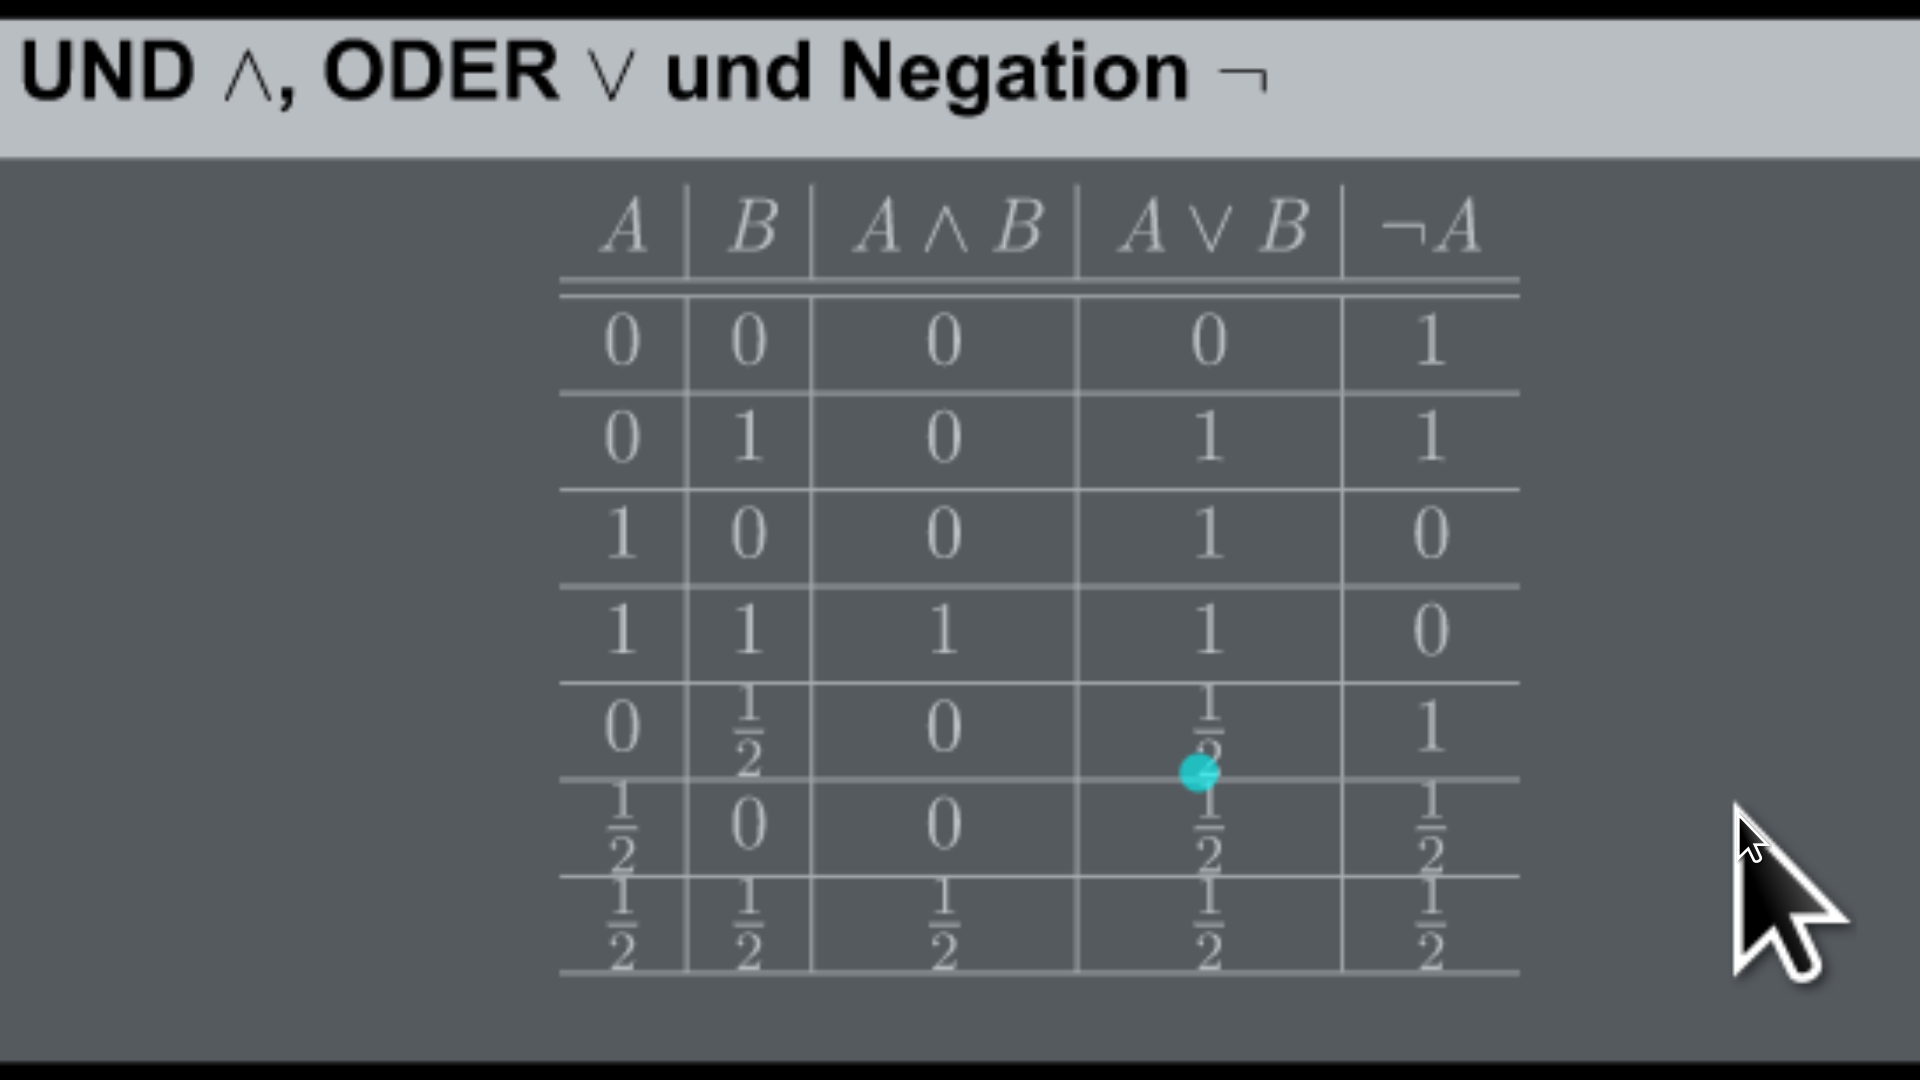
\includegraphics[width=\linewidth]{newtab} \\
	Wahrheitswerte Tabelle ändert sich mit null. \\
	unbekannt bekommt dabei den Wert $\frac{1}{2}$. \\
	null ist die Value in den Daten, unbekannt ist dessen Wahrheitswert. \\
	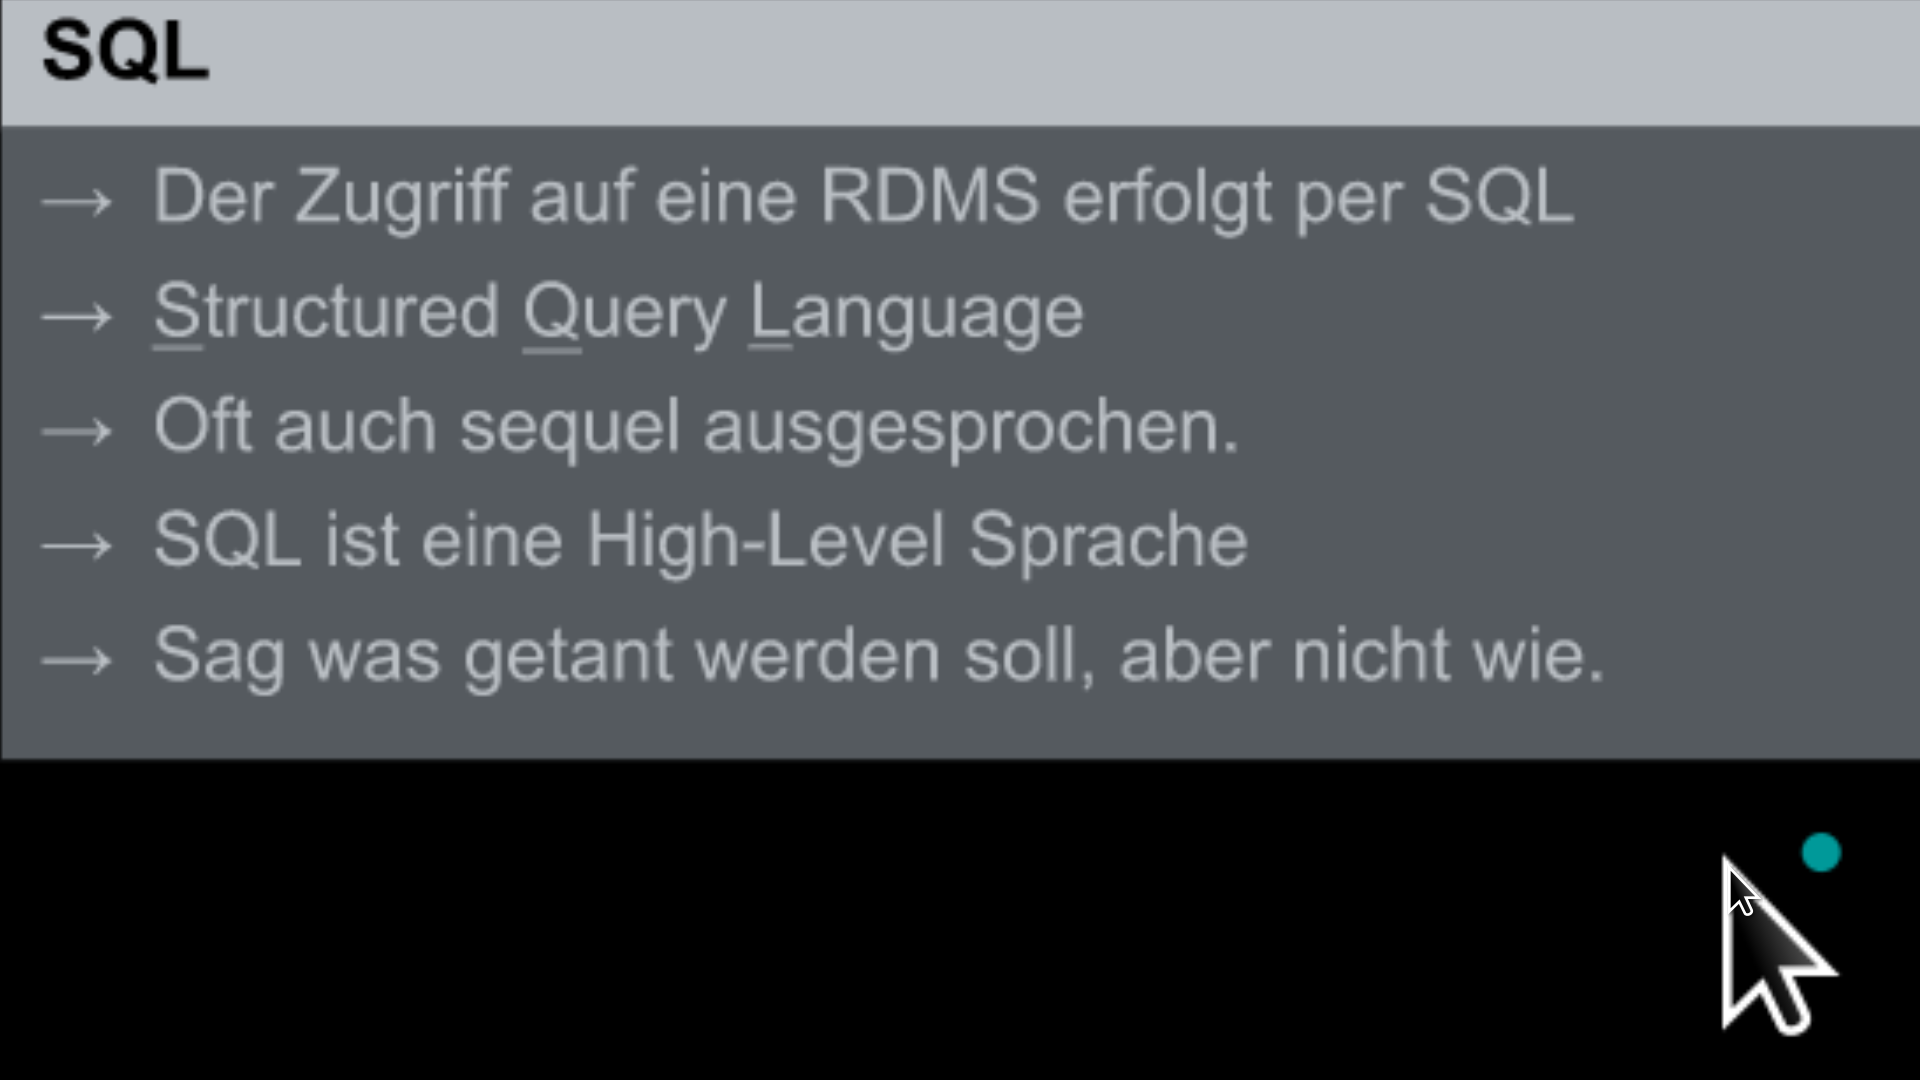
\includegraphics[width=\linewidth]{sql}
	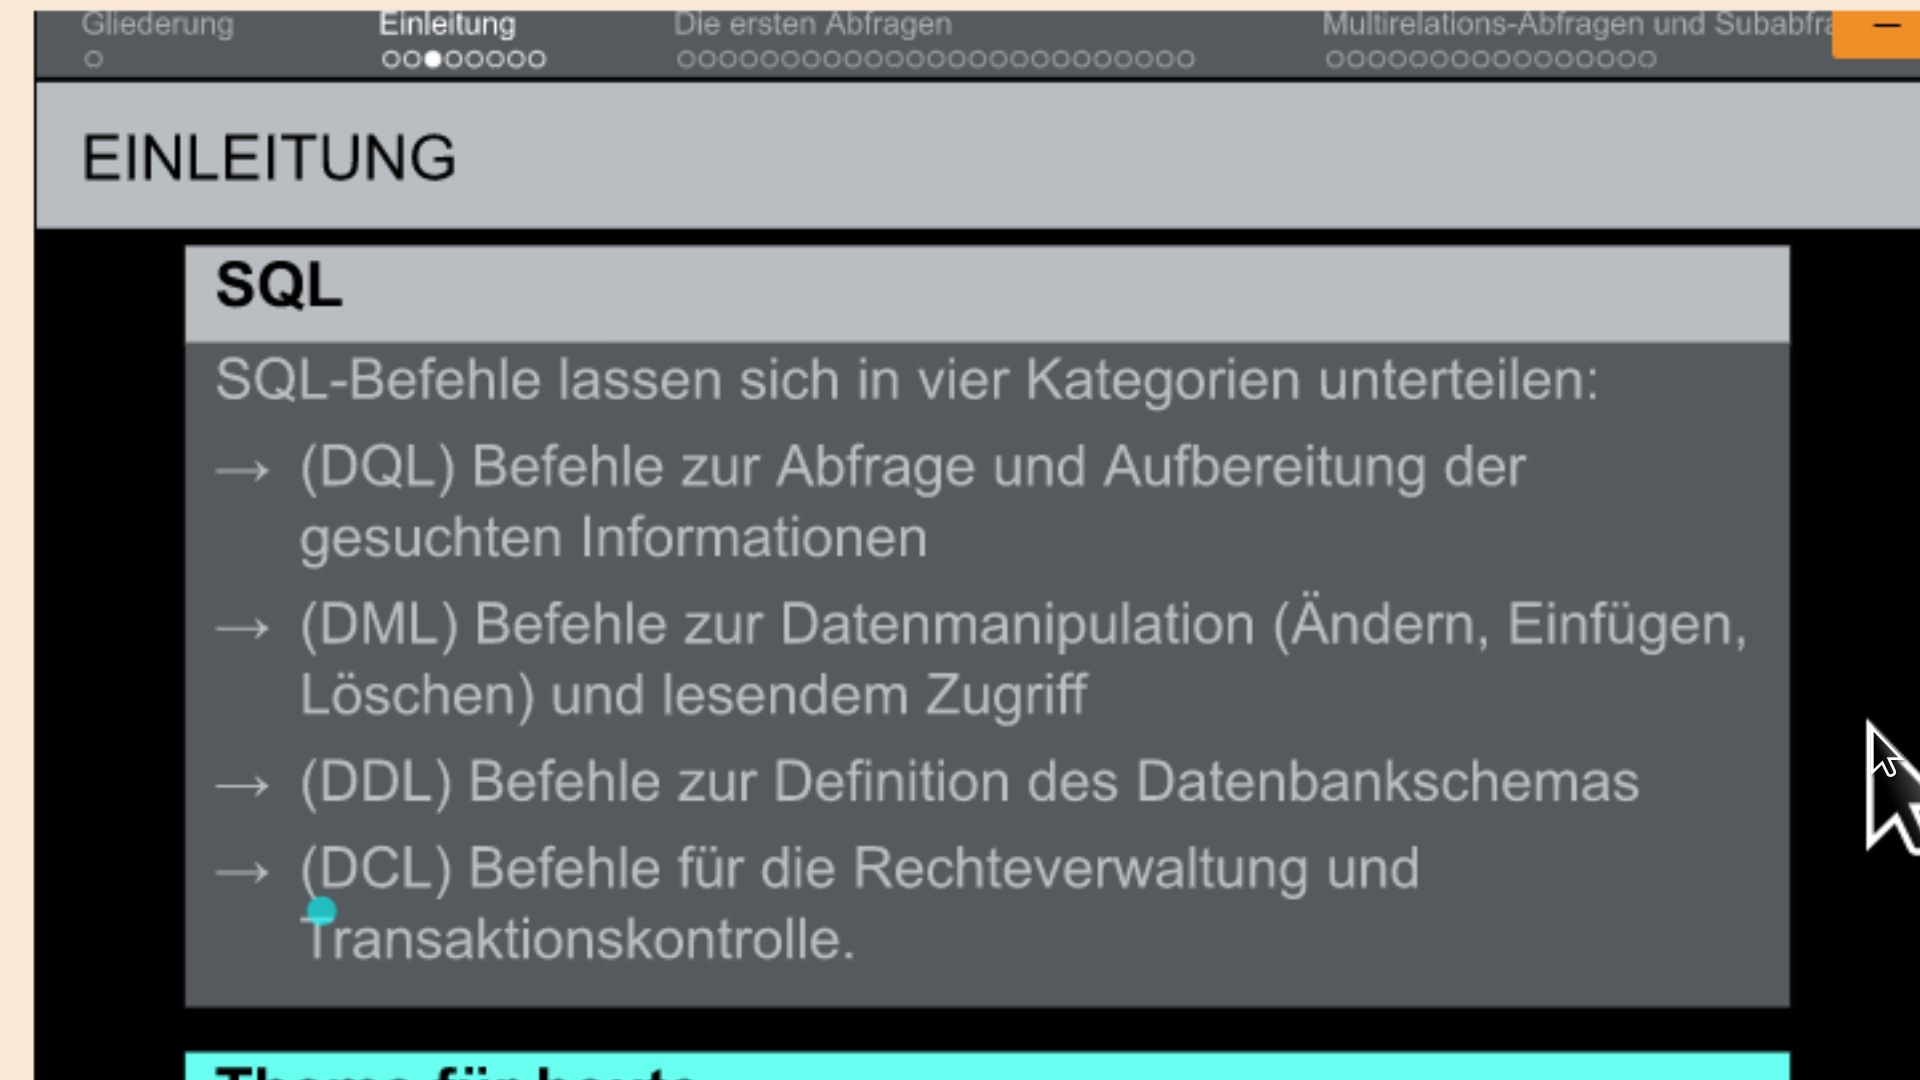
\includegraphics[width=\linewidth]{lang} \\
	\subsection*{10.06.2021}
	Entethy relationship modell \\
	Entitäten = Objekte \\
	Objekte haben Attribute \\
	Entity-Set Menge von Objekten \\
	Entität hat zwingend einen Schlüssel, der jedes Tupel identifizieren kann. \\
	Vermeidung von Redundanz \\
	Beziehung zu Entitäten \\
	1:n, n:n, n:1, 1:1 \\
	Kardinalitäten \\
	1:m 1 Leser leiht n Bücher aus \\
	schwache Entität \\
	keinen Identitiver gefunden. \\
	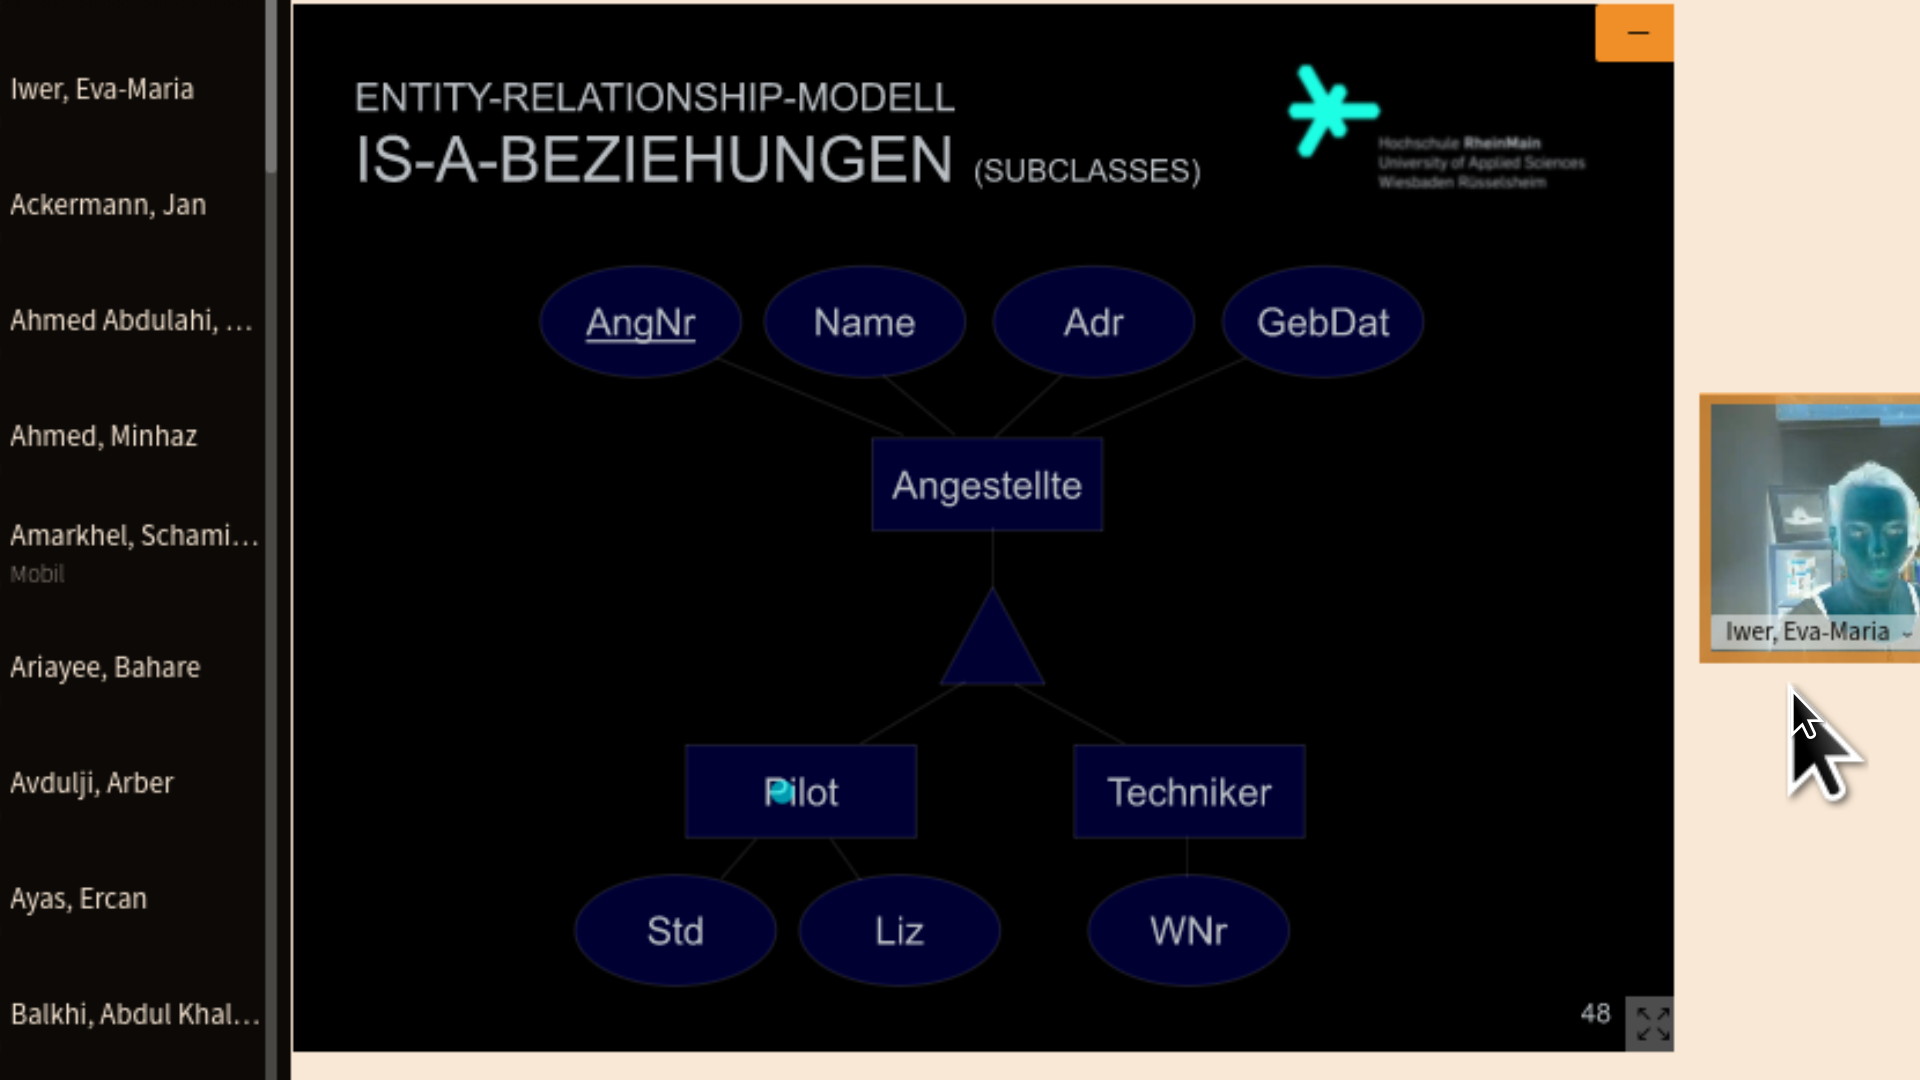
\includegraphics[width=\linewidth]{subclass} \\
	partielle und totale Ordnung \\
	total: Entscheiden entweder oder \\
	partielle Ordnung musst dich nicht entscheiden. \\
	\subsection*{17.06.2021}
	ERM \\
	Entitäten totale Unterteilung \\
	Attribute: Beschreibung einer Entität \\
	Nur Hauptklasse braucht Schlüssel \\
	Subklasse erbt Eigenschaften der Subklasse \\
	
\includegraphics[width=\linewidth]{erq} \\
	Kommunikation und Dokumentation  \\
	Maximal eine Dreierbeziehung \\
	möglichst natürliche Schlüssel \\
	wenig Redundanzen \\
	Jedes Entity hat eine Verbindung \\
	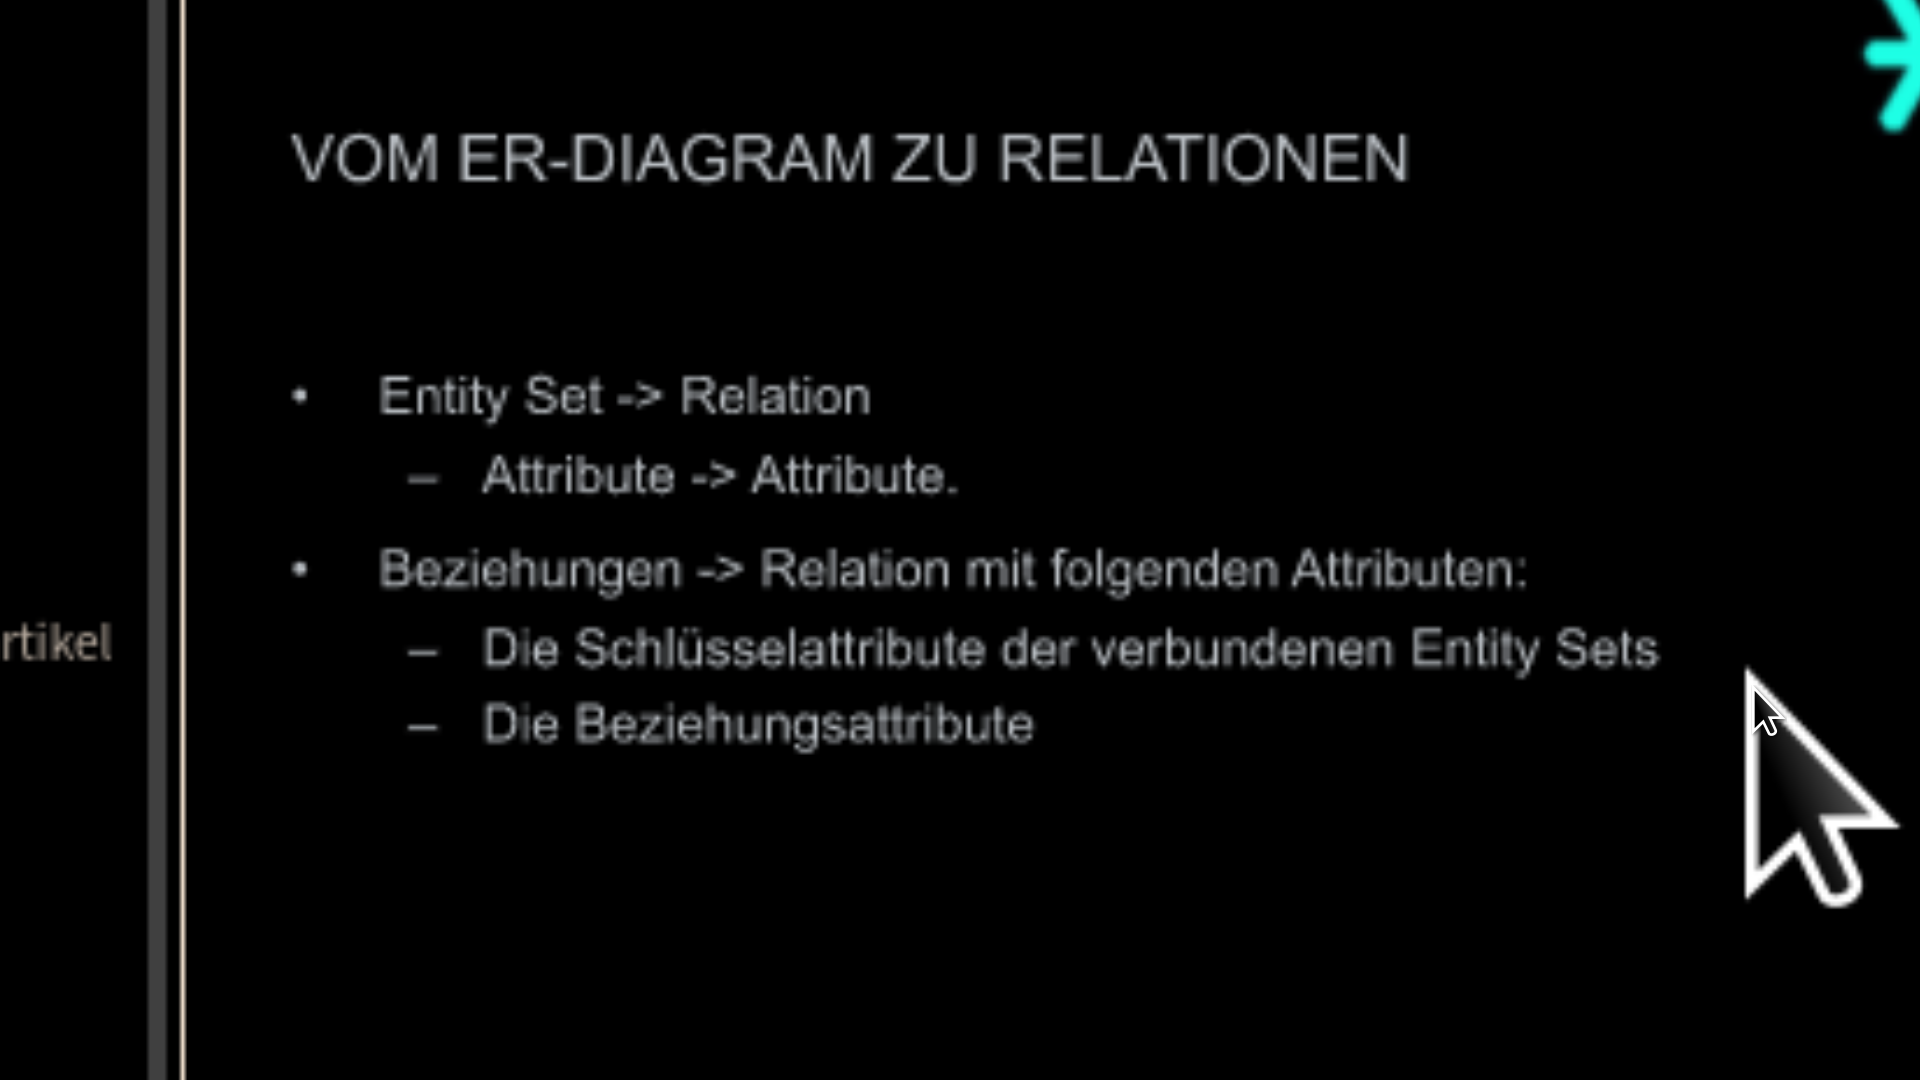
\includegraphics[width=\linewidth]{etr} \\
	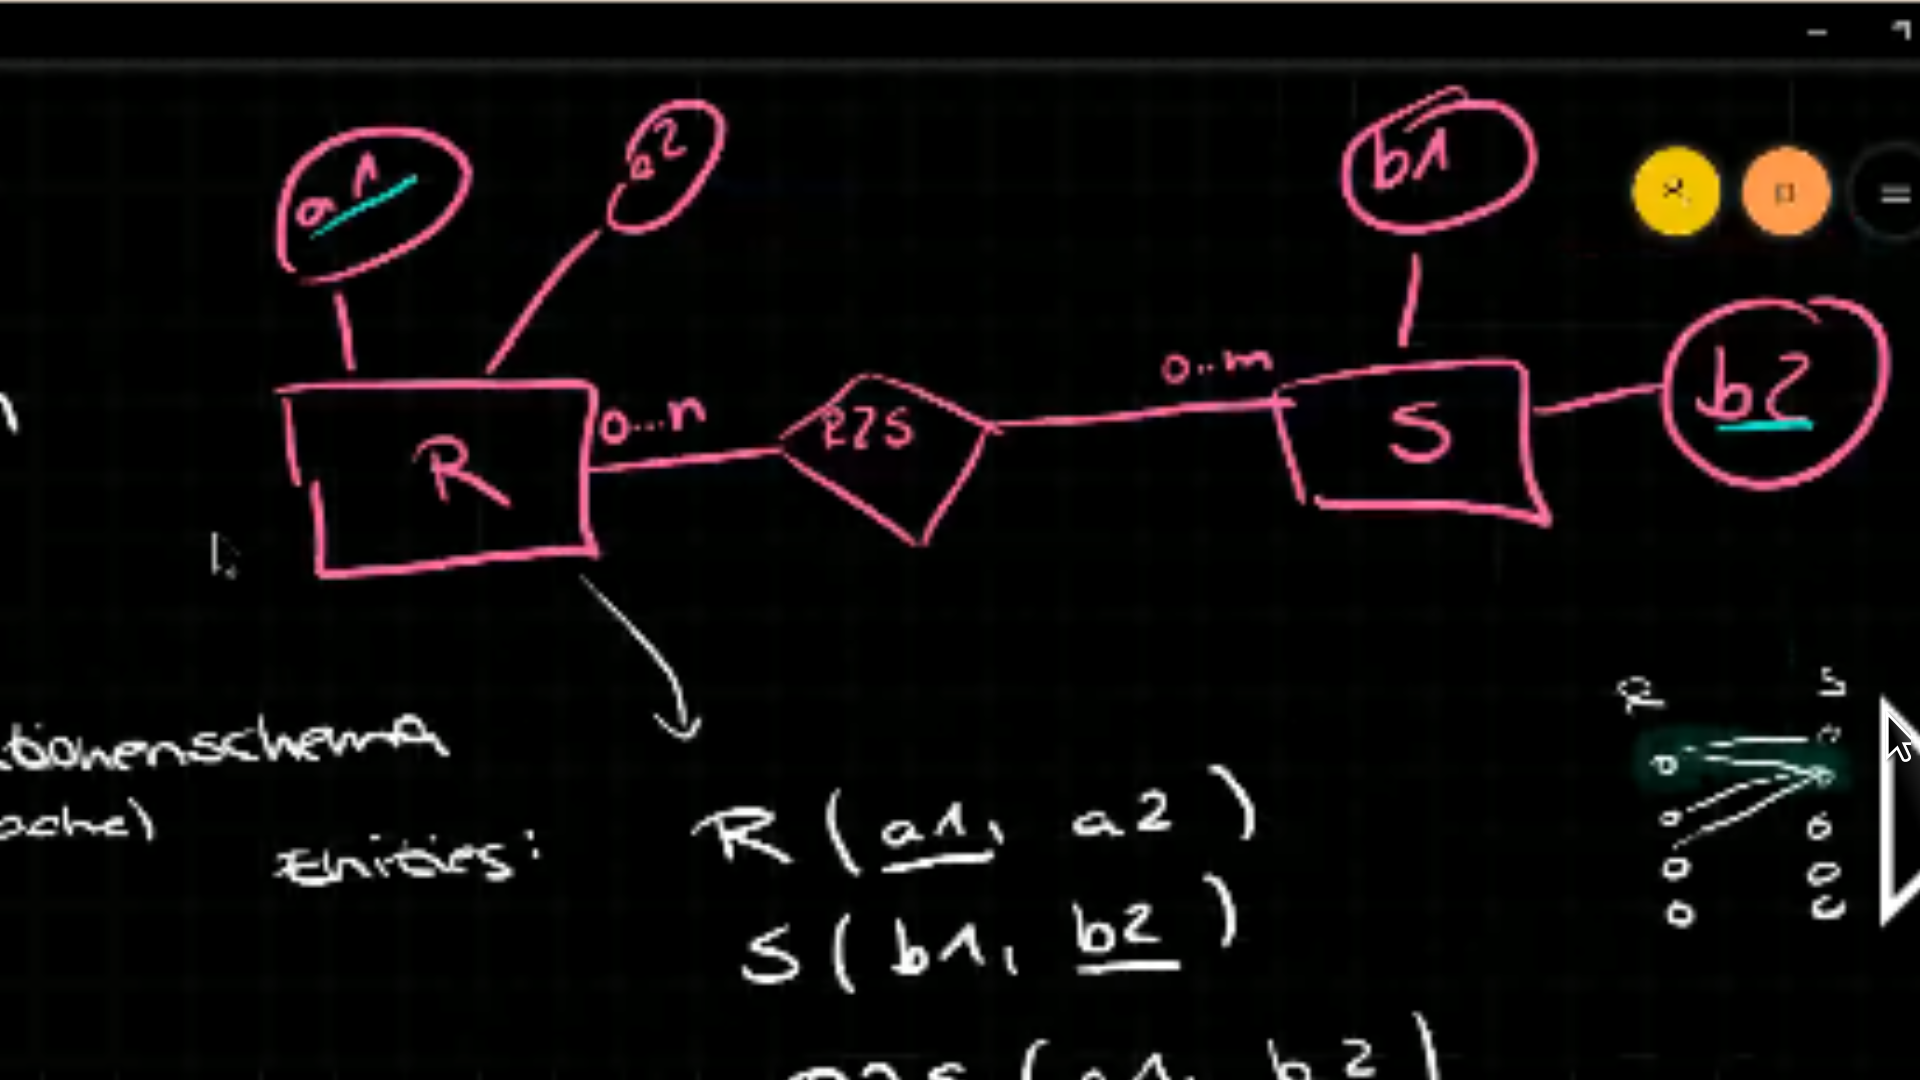
\includegraphics[width=\linewidth]{etr2} \\
	SQL DML\\
	Primär- und Fremdschlüssel beachten \\
	Integrationsbedingunen bei Definition festlegen \\
	Cascade \\
	View virtuelle Tabelle \\
	\subsection*{24.06.2021}
	Primary Key für Eindeutigkeit \\
	Fremdschlüssel sehr wichtig \\
	Trigger \\
	IF-Statment absetzen bei Datenbankaufruf \\
	Bei 1:1 Beziehung über Attribut nachdenken \\
	\subsection*{01.07.2021}
	Kapselung von SQL Kommandos \\
	entweder alle Kommandos werden ausgeführt. Wenn ein Befehl fehlschlägt werden alle Befehle rückgängig machen. \\
	ACID \\
	Transaktion endet mit COMMIT oder ROLEBACK \\
	SAVEPOINT Speicherpunkt innerhalb der Transaktion \\
	Datensicherungssprung \\
	Datenlage wird zurückgesetzt \\
	
\end{document}